\chapter{Weakly Interacting Bose Gas}

\section{The Weak Interaction Assumption}

The weakly interacting Bose gas serves as a foundational paradigm in quantum many-body theory. We consider a system of \( N \) identical bosons of mass \( m \) confined to a box of volume \( V = L^3 \) with periodic boundary conditions.

The interparticle interaction is characterized by a two-body potential \( U(\mathbf{r}) \), which we assume to be weak. The constituents of this gas obey Bose-Einstein statistics and are treated as non-relativistic elementary particles, meaning that their internal degrees of freedom are not activated at the relevant energy scales, and the total particle number is strictly fixed (precluding, for example, a gas of photons).

\begin{figure}[H]
    \centering
    \begin{minipage}{0.55\textwidth}
        \centering
        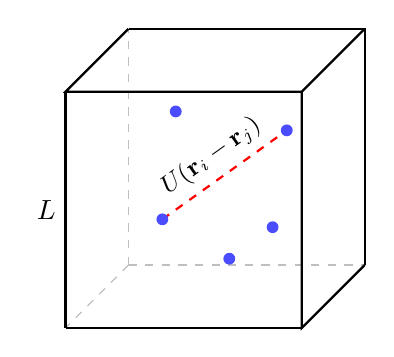
\begin{tikzpicture}[x=1.5cm, y=1.5cm, z={(-0.4cm, -0.4cm)}, scale=1]
            \def\L{2}

            \draw[gray!50, dashed] (0,0,0) -- (0,\L,0);
            \draw[gray!50, dashed] (0,0,0) -- (\L,0,0);
            \draw[gray!50, dashed] (0,0,0) -- (0,0,\L);

            \coordinate (A1) at (0.5, 0.6, 0.8);
            \coordinate (A2) at (1.5, 1.3, 0.6);
            \coordinate (A3) at (0.8, 1.7, 1.5);
            \coordinate (A4) at (1.2, 0.4, 1.3);
            \coordinate (A5) at (1.7, 0.8, 1.8);

            \draw[dashed, red, thick] (A1) -- (A2)
            node[midway, above, sloped, black] {\small $U(\mathbf{r}_i - \mathbf{r}_j)$};

            \foreach \p in {A1, A2, A3, A4, A5} {
                    \fill[blue!70] (\p) circle (0.05);
                }

            \draw[thick] (\L,0,0) -- (\L,\L,0) -- (0,\L,0);
            \draw[thick] (0,\L,0) -- (0,\L,\L) -- (\L,\L,\L) -- (\L,\L,0);
            \draw[thick] (\L,0,0) -- (\L,0,\L) -- (\L,\L,\L);
            \draw[thick] (0,0,\L) -- (\L,0,\L);
            \draw[thick] (0,0,\L) -- (0,\L,\L);

            \node[left] at (0, \L/2, \L) {$L$};

        \end{tikzpicture}
    \end{minipage}\hfill
    \begin{minipage}{0.4\textwidth}
        \caption{Schematic representation of a system of $N$ interacting bosons confined within a cubic box of volume $V=L^3$. The periodic boundary conditions simulate a bulk system. The dashed red line illustrates the two-body interaction potential $U(\mathbf{r}_i - \mathbf{r}_j)$ acting strictly between pairs of particles.}
        \label{fig:bose_gas_box}
    \end{minipage}
\end{figure}

Typical experimental realizations involve dilute gases of bosonic atoms, meaning atoms possessing an even total number of constituent fermions (protons, neutrons, and electrons), such as Sodium (\( ^{23}\text{Na} \)), Rubidium (\( ^{87}\text{Rb} \)), Potassium (\( ^{41}\text{K} \)), Cesium (\( ^{133}\text{Ce} \)), and Lithium (\( ^{7}\text{Li} \)). Historically, this theoretical framework was first motivated by efforts to explain the superfluid behavior of Helium-4 below \( 2.17\text{K} \), despite the fact that liquid \( ^{4}\text{He} \) actually resides in a strongly interacting regime.

The Hamiltonian governing this system of \( N \) interacting identical bosons is given in first quantization by
\[
    \hat{H} = \sum_{i=1}^N \frac{\hat{\mathbf{p}}_i^2}{2m} + \frac{1}{2} \sum_{\substack{i,j \\ i \neq j}} U(\hat{\mathbf{r}}_i - \hat{\mathbf{r}}_j),
\]
where \( \hat{\mathbf{p}}_i \) is the momentum operator of the \( i \)-th particle, and \( U(\hat{\mathbf{r}}_i - \hat{\mathbf{r}}_j) \) represents the interaction energy between the \( i \)-th and \( j \)-th particles.

For a system comprising a macroscopic number of identical bosons, it is highly advantageous to transition to the second quantization formalism.\footnote{For a very clear introduction to the second quantization formalism for many-particle systems, see: H. Tasaki, \url{https://arxiv.org/pdf/1812.10732v5}.} We introduce bosonic creation and annihilation operators associated with the momentum eigenfunctions of a single particle. For a box with periodic boundary conditions, these single-particle states are quantized plane waves:
\[
    \phi_{\mathbf{k}}(\mathbf{r}) = \frac{e^{i \mathbf{k} \cdot \mathbf{r}}}{\sqrt{V}},
\]
where the allowed wave vectors \( \mathbf{k} \) take the discrete values
\[
    \mathbf{k} = \frac{\pi}{L} (n_x, n_y, n_z), \quad n_x, n_y, n_z \in \{0, \pm 1, \pm 2, \dots \}.
\]
In this momentum basis, the many-body Hamiltonian becomes
\begin{equation} \label{eq:ham_second_quant}
    \hat{H} = \sum_{\mathbf{k}} \epsilon_k \hat{a}^\dagger_{\mathbf{k}} \hat{a}_{\mathbf{k}} + \frac{1}{2V} \sum_{\mathbf{k}, \mathbf{k}', \mathbf{q}} U(\mathbf{q}) \hat{a}^\dagger_{\mathbf{k}+\mathbf{q}} \hat{a}^\dagger_{\mathbf{k}'-\mathbf{q}} \hat{a}_{\mathbf{k}'} \hat{a}_{\mathbf{k}}.
\end{equation}
Here, \( \epsilon_k \) denotes the non-interacting energy associated with the wave vector \( \mathbf{k} \) (which depends exclusively on its magnitude \( k \)), given by the free-particle dispersion
\[
    \epsilon_k = \frac{\hbar^2 k^2}{2m},
\]
and \( U(\mathbf{q}) \) is the Fourier transform of the real-space two-body potential \( U(\hat{\mathbf{r}}_1 - \hat{\mathbf{r}}_2) \). The operators \( \hat{a}_{\mathbf{k}}^\dagger \) and \( \hat{a}_{\mathbf{k}} \) represent the creation and destruction operators for the corresponding momentum eigenstates.

In the idealized limit where interactions are completely absent, the ground state of the system is trivial: all \( N \) bosons condense into the lowest-energy single-particle state featuring zero momentum (\( \mathbf{k} = 0 \)). This macroscopic formation of a condensate is mathematically expressed by acting \( N \) times with the zero-momentum creation operator \( \hat{a}_0^\dagger \) on the vacuum state \( \ket{0} \) (incorporating the standard \( 1/\sqrt{N!} \) normalization factor for formal completeness):
\begin{equation} \label{eq:ideal_bec}
    \ket{\psi_0^{(0)}} = \frac{(\hat{a}_0^\dagger)^N}{\sqrt{N!}}  \ket{0}.
\end{equation}


\begin{remark}
    This clustering phenomenon stands in stark contrast to the behavior of a gas of fermions. Governed by the Pauli exclusion principle, fermions are strictly forbidden from occupying identical quantum states. Consequently, even at zero temperature, non-interacting fermions must sequentially fill all available momentum states up to a maximum threshold known as the Fermi energy, precluding any analogous zero-momentum condensation.
\end{remark}

We now introduce the principal assumption of our approach: the interparticle interaction is sufficiently weak. Given this, we anticipate that the true, interacting ground state remains a modest perturbation of the unperturbed condensate state \( \ket{\psi_0^{(0)}} \). Therefore, even in the presence of interactions, the vast majority of the bosons will remain in the zero-momentum single-particle state. This physical condition is formalized by the inequality
\begin{equation} \label{eq:weak_interaction_condition}
    \frac{N - N_0}{N} \ll 1,
\end{equation}
where \( N_0 = \langle \hat{a}^\dagger_0 \hat{a}_0 \rangle \) defines the thermodynamic average number of bosons residing in the condensate. The quantity \( N - N_0 \) thus counts the number of depleted bosons that have been excited out of the condensate into states with \( \mathbf{k} \neq 0 \). Due to the weakness of the interaction, these non-zero momentum states are only microscopically occupied, meaning their occupation numbers scale as \( \langle \hat{a}^\dagger_{\mathbf{k}} \hat{a}_{\mathbf{k}} \rangle = \mathcal{O}(1) \). Crucially, the population of these excited states does not scale proportionally with the macroscopic total particle number \( N \).

We leverage this assumption to implement a fundamental approximation on the interaction term of the Hamiltonian \eqref{eq:ham_second_quant}. Because operators acting on the condensate (\( \hat{a}_0 \) and \( \hat{a}^\dagger_0 \)) scale macroscopically with \( \sqrt{N_0} \approx \sqrt{N} \), we can safely neglect all interaction terms containing more than two operators equipped with non-zero momentum (\( \hat{a}_{\mathbf{k}} \) or \( \hat{a}^\dagger_{\mathbf{k}} \) for \( \mathbf{k} \neq 0 \)). (Note that terms containing exactly three zero-momentum operators are inherently forbidden by momentum conservation requirements).

The most substantial and relevant term that survives this truncation is the one containing exclusively operators acting on the condensate (\( \mathbf{q} = 0 \) and \( \mathbf{k} = \mathbf{k}' = 0 \)):
\[
    \frac{1}{2V} U(\mathbf{q}=0) \hat{a}_0^\dagger \hat{a}_0^\dagger \hat{a}_0 \hat{a}_0 = \frac{1}{2V} U(\mathbf{q}=0) (\hat{N}_0^2 - \hat{N}_0).
\]

In the thermodynamic limit, \( \hat{N}_0 \) diverges linearly with \( N \). Thus, we can completely disregard the trailing \( \hat{N}_0 \) term in the above expression, as it scales infinitely slower than the dominant quadratic term \( \hat{N}_0^2 \sim N^2 \).

To systematically express this leading-order contribution in terms of the conserved total particle number, we recognize that the number of bosons in the ground state can be written as the difference between the total number operator \( \hat{N} \) and the sum of occupation numbers for all excited states:
\[
    \hat{N}_0 = \hat{N} - \sum_{\mathbf{k} \neq 0} \hat{a}^\dagger_{\mathbf{k}} \hat{a}_{\mathbf{k}},
\]
where the primed summation specifically denotes a sum over all allowed momenta excluding zero. Letting \( U_0 \equiv U(\mathbf{q}=0) \), we substitute this relation back into our dominant interaction term. Expanding the square and purposefully discarding the resulting quartic term (which contains four out-of-condensate operators and is therefore negligible under our approximation), we obtain
\[
    \frac{1}{2V} U_0 (\hat{N}_0)^2 = \frac{1}{2V} U_0 \left( \hat{N} - \sum_{\mathbf{k} \neq 0} \hat{a}^\dagger_{\mathbf{k}} \hat{a}_{\mathbf{k}} \right)^2 \approx \frac{1}{2V} U_0 \left( \hat{N}^2 - 2\hat{N} \sum_{\mathbf{k} \neq 0} \hat{a}^\dagger_{\mathbf{k}} \hat{a}_{\mathbf{k}} \right).
\]

Through this procedure, we successfully reduce the pure zero-momentum interaction into a quadratic form that couples the macroscopic total number \( N \) with the single-particle excitations.


\subsubsection{Quadratic Interaction Terms and the Short-Range Assumption}

Besides the dominant term where all operators are in the condensate state, we must evaluate the terms from the interaction Hamiltonian that contain exactly two operators with momentum different from zero. Before explicitly listing them, we introduce a crucial physical approximation: we replace the momentum-dependent interaction potential \( U(\mathbf{q}) \) with a simple constant, \( U(0) \).

This approximation is mathematically justified if the real-space potential is effectively ``short-ranged''. For the Fourier transform \( U(\mathbf{q}) = \int \mathrm{d}^3\mathbf{r} U(\mathbf{r}) e^{-i\mathbf{q}\cdot\mathbf{r}} \) to be well-behaved and approximately constant for small momenta, its zero-momentum limit \( U(0) = \int \mathrm{d}^3\mathbf{r} U(\mathbf{r}) \) must be finite. In three spatial dimensions, the spherical integration measure introduces a factor of \( r^2 \). Consequently, for the integral \( \int dr r^2 U(r) \) to converge at large interparticle distances, the potential \( U(r) \) must decay strictly faster than \( 1/r^3 \).

This convergence criterion dictates which physical systems can be described by this simplified model. In dilute atomic gases, van der Waals forces serve as an excellent example of a valid short-ranged potential. In the standard Lennard-Jones model, the long-range attractive tail scales as \( 1/r^6 \). Since \( 6 > 3 \), it comfortably satisfies the convergence requirement. In contrast, dipole-dipole interactions scale exactly as \( 1/r^3 \). This is a tricky marginal case where the spatial integral diverges logarithmically, meaning dipole interactions are mathematically long-ranged in 3D and cannot be treated with this simple approximation. Assuming our potential decays fast enough, we can safely set \( U(\mathbf{q}) \approx U(\mathbf{q}=0) \equiv U_0 \), making all subsequent calculations significantly simpler.

\begin{remark}
    As an analogous example of effective short-range interactions from high-energy physics, the strong nuclear force is also effectively short-ranged (decaying exponentially, much faster than \( 1/r^3 \)) because its mediators, pions, are massive.
\end{remark}

With the assumption \( U(\mathbf{q}) \approx U_0 \) established, we retain the following six terms containing exactly two non-zero momentum operators:

\begin{enumerate}
    \item If \( \mathbf{k} + \mathbf{q} = 0 \) and \( \mathbf{k}' - \mathbf{q} = 0 \), we have that \( \mathbf{k} = -\mathbf{q} \) and \( \mathbf{k}' = \mathbf{q} \), and so we remain with
          \[
              \frac{1}{2V} U_0 a_0^\dagger a_0^\dagger \sum_{\mathbf{q}}' a_{\mathbf{q}} a_{-\mathbf{q}},
          \]
          where the sum \( \sum_{\mathbf{q}}' \) is over all possible momenta \( \mathbf{q} \neq 0 \) because the zero case has been already taken into account in the previous purely macroscopic term.

    \item If \( \mathbf{k} + \mathbf{q} = 0 \) and \( \mathbf{k}' = 0 \), using again the short-range assumption, the term takes the following form:
          \[
              \frac{1}{2V} U_0 \sum_{\mathbf{q}}' a_0^\dagger a_{-\mathbf{q}}^\dagger a_0 a_{-\mathbf{q}} = \frac{1}{2V} U_0 a_0^\dagger a_0 \sum_{\mathbf{q}}' a_{-\mathbf{q}}^\dagger a_{-\mathbf{q}}.
          \]

    \item If \( \mathbf{k} + \mathbf{q} = 0 \) and \( \mathbf{k} = 0 \), and so \( \mathbf{q} = 0 \), we get
          \[
              \frac{1}{2V} U_0 \sum_{\mathbf{k}'}' a_0^\dagger a_{\mathbf{k}'}^\dagger a_{\mathbf{k}'} a_0 = \frac{1}{2V} U_0 a_0^\dagger a_0 \sum_{\mathbf{k}'}' a_{\mathbf{k}'}^\dagger a_{\mathbf{k}'}.
          \]

    \item If \( \mathbf{k}' - \mathbf{q} = 0 \) and \( \mathbf{k}' = 0 \), and so \( \mathbf{q} = 0 \), we get
          \[
              \frac{1}{2V} U_0 \sum_{\mathbf{k}}' a_{\mathbf{k}}^\dagger a_0^\dagger a_0 a_{\mathbf{k}} = \frac{1}{2V} U_0 a_0^\dagger a_0 \sum_{\mathbf{k}}' a_{\mathbf{k}}^\dagger a_{\mathbf{k}}.
          \]

    \item If \( \mathbf{k}' - \mathbf{q} = 0 \) and \( \mathbf{k} = 0 \), with the short-range assumption the term takes the following form:
          \[
              \frac{1}{2V} U_0 \sum_{\mathbf{q}}' a_{\mathbf{q}}^\dagger a_0^\dagger a_{\mathbf{q}} a_0 = \frac{1}{2V} U_0 a_0^\dagger a_0 \sum_{\mathbf{q}}' a_{\mathbf{q}}^\dagger a_{\mathbf{q}}.
          \]

    \item If \( \mathbf{k}' = 0 \) and \( \mathbf{k} = 0 \), with the short-range assumption the term takes the following form:
          \[
              \frac{1}{2V} U_0 \sum_{\mathbf{q}}' a_{\mathbf{q}}^\dagger a_{-\mathbf{q}}^\dagger a_0 a_0 = \frac{1}{2V} U_0 a_0 a_0 \sum_{\mathbf{q}}' a_{\mathbf{q}}^\dagger a_{-\mathbf{q}}^\dagger.
          \]
\end{enumerate}

\subsubsection{Condensate Mean-Field Approximation and the Bogoliubov Hamiltonian}

A further crucial step is the replacement of the operators \( a_0 \) and \( a_0^\dagger \) with numbers. Because the non-interacting ground state exhibits macroscopic occupation, its expectation value is \( \langle a_0^\dagger a_0 \rangle = N_0 \approx N \). Therefore, we can confidently approximate \( a_0 \sim \sqrt{N} \) and \( a_0^\dagger \sim \sqrt{N} \) across all the previously derived terms of the approximate Hamiltonian that contain two condensate operators multiplied by two out-of-condensate operators.\footnote{This can be preatty disturbing, since the expectation value of a single ladder operator is usually zero; but, as we will see later, we are not using eigenstates of number operator, instead superpositions of those (similar to coherent states). Indeed, even if the hamiltonian conserves the number of particle, the ground state description does not really rely on a fixed occupation of bosons. We will stress this point later on.}

This mean-field approximation is formally justified by inspecting the commutator \( [a_0, a_0^\dagger] = 1 \) and comparing its magnitude to the result of acting with these operators on the non-interacting \( N \)-particle ground state \( \ket{\psi_0^{(0)}(N)} \). Specifically, one finds:
\[
    a_0 \ket{\psi_0^{(0)}(N)} = \sqrt{N} \ket{\psi_0^{(0)}(N-1)} \sim \sqrt{N} \ket{\psi_0^{(0)}(N)},
\]
and
\[
    a_0^\dagger \ket{\psi_0^{(0)}(N)} = \sqrt{N+1} \ket{\psi_0^{(0)}(N+1)} \sim \sqrt{N} \ket{\psi_0^{(0)}(N)},
\]
where we have safely neglected \( 1 \) relative to the macroscopically large number \( N \) in these expressions. Because of this scaling, the value of the commutator is entirely negligible, and the operators can be effectively treated as commuting c-numbers.

Furthermore, during this systematic expansion, it is important to recognize why linear terms in \( a_{\mathbf{k}} \) or \( a_{\mathbf{k}}^\dagger \) do not appear. The terms which cancel out are precisely the ones that contain a single \( \hat{a}_0 \) or \( \hat{a}_0^\dagger \) in the interaction term; if they did not cancel, they would have contributed to an unphysical renormalization of the free term of the Hamiltonian.

By substituting these numerical expectations back into our aggregated interaction terms, the full Hamiltonian becomes:\TODO{expand computations.}
\begin{equation} \label{eq:bogoliubov_hamiltonian}
    H = \sum_{\mathbf{k}}' (\epsilon_k + nU_0) a_{\mathbf{k}}^\dagger a_{\mathbf{k}} + \frac{nU_0}{2} \sum_{\mathbf{k}}' (a_{-\mathbf{k}}^\dagger a_{\mathbf{k}}^\dagger + a_{\mathbf{k}} a_{-\mathbf{k}}) + \frac{1}{2}V n^2 U_0,
\end{equation}
where \( n = N/V \) is the particle density.

Note that the second sum in the above equation contains the ``anomalous'' terms \( a_{-\mathbf{k}}^\dagger a_{\mathbf{k}}^\dagger \) and \( a_{\mathbf{k}} a_{-\mathbf{k}} \). Because the Hamiltonian now pairs creation operators together (and annihilation operators together) rather than consisting purely of standard number operators, it is not diagonal. To resolve this and find the true elementary excitations, one must employ the Bogoliubov transformation to diagonalize the Hamiltonian.

As a final remark, we note that if one were to carry out this derivation without invoking the constant potential approximation \( U(\mathbf{q}) \simeq U_0 \), the resulting Hamiltonian would naturally retain the momentum dependence of the interaction:
\[
    H = \sum_{\mathbf{k}}' (\epsilon_k + nU(k)) a_{\mathbf{k}}^\dagger a_{\mathbf{k}} + \frac{n}{2} \sum_{\mathbf{k}}' U(k) (a_{-\mathbf{k}}^\dagger a_{\mathbf{k}}^\dagger + a_{\mathbf{k}} a_{-\mathbf{k}}) + \frac{1}{2}V n^2 U_0.
\]

\subsubsection{Summary of Assumptions and Approximations}

Before proceeding to diagonalize the Hamiltonian, it is instructive to summarize the hierarchy of physical assumptions and mathematical approximations that have systematically reduced the complex many-body problem to the quadratic Bogoliubov Hamiltonian \eqref{eq:bogoliubov_hamiltonian}:

\begin{itemize}
    \item \textbf{Non-Relativistic Elementary Bosons:} We assume the particles are massive, non-relativistic, and constrained to energy scales where internal degrees of freedom are completely frozen.
          \textit{Consequence:} The total particle number \( N \) is strictly conserved (unlike in a photon gas), and the system is well-described by standard Galilean kinetic energy and a static scalar two-body potential.

    \item \textbf{Weak Interaction Hypothesis:} The interparticle potential is assumed to be sufficiently weak such that the true interacting ground state is only a modest perturbation of the ideal Bose-Einstein condensate.
          \textit{Consequence:} The fraction of depleted particles is vanishingly small (\( (N-N_0)/N \ll 1 \)). This justifies truncating the interaction Hamiltonian to discard all terms containing more than two out-of-condensate operators (\( \mathbf{k} \neq 0 \)).

    \item \textbf{Short-Range Potential:} The two-body interaction \( U(\mathbf{r}) \) is assumed to decay strictly faster than \( 1/r^3 \) at large interparticle distances.
          \textit{Consequence:} The Fourier transform of the potential converges and varies slowly at small momenta, allowing us to approximate \( U(\mathbf{q}) \approx U(\mathbf{q}=0) \equiv U_0 \). This dramatically simplifies the scattering amplitudes in the dilute gas regime.

    \item \textbf{Macroscopic Condensate Occupation (Mean-Field Limit):} The zero-momentum state is macroscopically occupied (\( N_0 \approx N \gg 1 \)), meaning the fundamental commutator \( [\hat{a}_0, \hat{a}_0^\dagger] = 1 \) is negligible compared to the absolute particle number.
          \textit{Consequence:} The macroscopic creation and annihilation operators \( \hat{a}_0^\dagger \) and \( \hat{a}_0 \) can be treated as commuting c-numbers and replaced by \( \sqrt{N} \). This breaks the \( U(1) \) phase symmetry of the Hamiltonian and reduces the complicated quartic interaction term into a tractable quadratic form featuring anomalous pairing terms.
\end{itemize}

\subsection{Bogoliubov Transformations}

We wish to diagonalize the Hamiltonian of the weakly interacting Bose gas by introducing new bosonic annihilation and creation operators, \( \alpha_{\mathbf{k}} \) and \( \alpha_{\mathbf{k}}^\dagger \), known as Bogoliubov operators. We need to construct a Hamiltonian which, in the end, depends only on a diagonal number operator of the form \( \alpha_{\mathbf{k}}^\dagger \alpha_{\mathbf{k}} \), yielding a target structure like:
\[
    H = \sum_{\mathbf{k}} E_k \alpha_{\mathbf{k}}^\dagger \alpha_{\mathbf{k}} + \text{const},
\]
for some energy dispersion \( E_k \). To eliminate the anomalous terms that mix creation and annihilation operators in our previous Hamiltonian, we can perform a Bogoliubov transformation, which is a linear transformation mapping the original particle operators to the new quasiparticle operators. We start with the following standard ansatz for the Bogoliubov transformation:
\begin{equation} \label{eq:bogoliubov_ansatz}
    \begin{dcases}
        \alpha_{\mathbf{k}} = u_k a_{\mathbf{k}} + v_k a_{-\mathbf{k}}^\dagger, \\
        \alpha_{\mathbf{k}}^\dagger = v_k^* a_{\mathbf{k}}^\dagger + u_k^* a_{-\mathbf{k}},
    \end{dcases}
\end{equation}
for \( \mathbf{k} \neq 0 \), where \( u_k \) and \( v_k \) are real coefficients. We now assume that these coefficients are real for simplicity, but they could in principle be complex.
These coefficients are defined to depend strictly on the momentum magnitude \( k = |\mathbf{k}| \), ensuring that rotational invariance is preserved in momentum space.

Because these newly defined operators must describe valid bosonic excitations, they are strictly required to satisfy the standard canonical bosonic commutation relations. We can verify this by evaluating the commutator between two annihilation operators:
\[
    \begin{aligned}
        [\alpha_{\mathbf{k}}, \alpha_{\mathbf{k}'}] = [u_k a_{\mathbf{k}} + v_k a_{-\mathbf{k}}^\dagger, u_{k'} a_{\mathbf{k}'} + v_{k'} a_{-\mathbf{k}'}^\dagger] \\
        = u_k v_{k'} [a_{\mathbf{k}}, a_{-\mathbf{k}'}^\dagger] + v_k u_{k'} [a_{-\mathbf{k}}^\dagger, a_{\mathbf{k}'}]                                            \\
        = u_k v_{k'} \delta_{\mathbf{k}, -\mathbf{k}'} - v_k u_{k'} \delta_{-\mathbf{k}, \mathbf{k}'} = 0,
    \end{aligned}
\]
which vanishes as expected. Next, we evaluate the critical commutator between a creation and an annihilation operator:
\[
    \begin{aligned}
        [\alpha_{\mathbf{k}}, \alpha_{\mathbf{k}'}^\dagger] = [u_k a_{\mathbf{k}} + v_k a_{-\mathbf{k}}^\dagger, u_{k'} a_{\mathbf{k}'}^\dagger + v_{k'} a_{-\mathbf{k}'}] \\
        = u_k u_{k'} [a_{\mathbf{k}}, a_{\mathbf{k}'}^\dagger] + v_k v_{k'} [a_{-\mathbf{k}}^\dagger, a_{-\mathbf{k}'}]                                                    \\
        = (u_k^2 - v_k^2)\delta_{\mathbf{k}, \mathbf{k}'}.
    \end{aligned}
\]
To enforce the correct commutation relations, we must impose a hyperbolic normalization condition on the coefficients:
\begin{equation} \label{eq:bogoliubov_condition}
    \vert u_k \vert^2 - \vert v_k\vert^2 = 1.
\end{equation}

Provided this condition holds, the transformation linking the old and new operators can be easily inverted. We can express the linear mapping and its Hermitian conjugate in matrix notation:
\[
    \begin{pmatrix} \alpha_{\mathbf{k}} \\ \alpha_{-\mathbf{k}}^\dagger \end{pmatrix} = \begin{pmatrix} u_k & v_k \\ v_k & u_k \end{pmatrix} \begin{pmatrix} a_{\mathbf{k}} \\ a_{-\mathbf{k}}^\dagger \end{pmatrix}.
\]
Because the determinant of the transformation matrix is exactly \( u_k^2 - v_k^2 = 1 \), the matrix is trivially invertible:
\[
    \begin{pmatrix} a_{\mathbf{k}} \\ a_{-\mathbf{k}}^\dagger \end{pmatrix} = \begin{pmatrix} u_k & -v_k \\ -v_k & u_k \end{pmatrix} \begin{pmatrix} \alpha_{\mathbf{k}} \\ \alpha_{-\mathbf{k}}^\dagger \end{pmatrix},
\]
which explicitly yields the inverted transformation:
\[
    \begin{dcases}
        a_{\mathbf{k}} = u_k \alpha_{\mathbf{k}} - v_k \alpha_{-\mathbf{k}}^\dagger, \\
        a_{\mathbf{k}}^\dagger = u_k \alpha_{\mathbf{k}}^\dagger - v_k \alpha_{-\mathbf{k}}.
    \end{dcases}
\]

We now proceed with the formal diagonalization of the Hamiltonian by expressing it entirely in terms of the new Bogoliubov operators:
\[
    H = \sum_{\mathbf{k}}' \left[ (\epsilon_k + nU_0)v_k^2 - nU_0 u_k v_k \right] + \frac{1}{2}Vn^2U_0
\]
\[
    + \sum_{\mathbf{k}}' \left[ (\epsilon_k + nU_0)(u_k^2 + v_k^2) - 2nU_0 u_k v_k \right] \alpha_{\mathbf{k}}^\dagger \alpha_{\mathbf{k}}
\]
\[
    + \sum_{\mathbf{k}}' \left[ \frac{nU_0}{2}(u_k^2 + v_k^2) - u_k v_k(\epsilon_k + nU_0) \right] (\alpha_{\mathbf{k}}^\dagger \alpha_{-\mathbf{k}}^\dagger + \alpha_{-\mathbf{k}} \alpha_{\mathbf{k}}).
\]
It may initially appear that we have not made significant progress, as the final line still contains non-diagonal anomalous terms. However, we now have the mathematical freedom to choose arbitrary coefficients that eliminate these specific terms. By selecting an appropriate \( v_k \) (which simultaneously determines \( u_k \) via the constraint \( u_k^2 = 1 + v_k^2 \)), we can force the bracketed prefactor of the off-diagonal terms to vanish identically:
\[
    \frac{nU_0}{2}(u_k^2 + v_k^2) - u_k v_k(\epsilon_k + nU_0) = 0.
\]
Through simple algebraic manipulation and applying our normalization condition, this requirement simplifies to a second-order polynomial equation for \( v_k^2 \):
\[
    4E_k^2 v_k^4 + 4E_k^2 v_k^2 - (nU_0)^2 = 0,
\]
where we have suggestively defined the factor \( E_k^2 \) as:
\begin{equation} \label{eq:bogoliubov_spectrum_squared}
    E_k^2 = (\epsilon_k + nU_0)^2 - (nU_0)^2.
\end{equation}
Solving this equation for \( v_k^2 \) directly yields the functional form of the transformation coefficients:
\[
    v_k^2 = \frac{1}{2} \left( \frac{\epsilon_k + nU_0}{E_k} - 1 \right),
\]
and consequently,
\[
    u_k^2 = \frac{1}{2} \left( \frac{\epsilon_k + nU_0}{E_k} + 1 \right),
\]
which implies for the cross-term:
\[
    u_k v_k = \frac{nU_0}{2E_k}.
\]

By inserting these rigorously derived coefficients back into our expanded operator expression, the off-diagonal terms strictly cancel, yielding the final form of the diagonalized Hamiltonian:
\begin{equation} \label{eq:diagonalized_hamiltonian}
    H = \sum_{\mathbf{k}}' E_k \alpha_{\mathbf{k}}^\dagger \alpha_{\mathbf{k}} + \mathcal{E}_0,
\end{equation}
where \( \mathcal{E}_0 \) is a macroscopic constant energy shift defined by:
\[
    \mathcal{E}_0 = \frac{1}{2}Vn^2U_0 - \frac{1}{2}\sum_{\mathbf{k}}' (\epsilon_k + nU_0 - E_k).
\]
The quantity \( E_k = [(\epsilon_k + nU_0)^2 - (nU_0)^2]^{1/2} > 0 \) represents the fundamental quasiparticle excitation spectrum of the system.

\subsubsection{The Non-Interacting Limit}

In the non-interacting limit, characterized by a vanishing interaction strength \( U_0 \to 0 \), it is instructive to verify that our diagonalized theory smoothly recovers the foundational physics of the ideal Bose gas.

First, we examine the Bogoliubov quasiparticle excitation spectrum \( E_k \). By taking the limit of the dispersion relation, we find:
\[
    E_k = \lim_{U_0 \to 0} \sqrt{(\epsilon_k + nU_0)^2 - (nU_0)^2} = \sqrt{\epsilon_k^2} = \epsilon_k.
\]
As physically expected, the quasiparticle spectrum trivially reduces to the free-particle kinetic energy \( \epsilon_k = \hbar^2 k^2 / (2m) \).

Next, we evaluate the asymptotic behavior of the Bogoliubov transformation coefficients \( v_k^2 \) and \( u_k^2 \). Substituting \( E_k \to \epsilon_k \) and \( U_0 \to 0 \), we obtain:
\[
    v_k^2 = \lim_{U_0 \to 0} \frac{1}{2} \left( \frac{\epsilon_k + nU_0}{E_k} - 1 \right) = \frac{1}{2}(1 - 1) = 0,
\]
and correspondingly,
\[
    u_k^2 = \lim_{U_0 \to 0} \frac{1}{2} \left( \frac{\epsilon_k + nU_0}{E_k} + 1 \right) = \frac{1}{2}(1 + 1) = 1.
\]
This implies that \( u_k \to 1 \) and \( v_k \to 0 \). Consequently, the Bogoliubov quasiparticle operators \( \alpha_{\mathbf{k}} = u_k a_{\mathbf{k}} + v_k a_{-\mathbf{k}}^\dagger \) reduce identically to the bare particle operators \( a_{\mathbf{k}} \). In the absence of interactions, the elementary excitations of the system are simply the original non-interacting bosons themselves, and the quantum depletion of the condensate drops to zero.

Finally, we analyze the macroscopic constant energy shift \( \mathcal{E}_0 \). The purely classical mean-field contribution \( \frac{1}{2}Vn^2U_0 \) obviously vanishes. For the quantum fluctuation sum, we note that \( E_k \approx \epsilon_k + nU_0 - \frac{(nU_0)^2}{2\epsilon_k} \) for small \( U_0 \), meaning the summand \( (\epsilon_k + nU_0 - E_k) \sim \mathcal{O}(U_0^2) \). Therefore, the entire shift vanishes:
\[
    \lim_{U_0 \to 0} \mathcal{E}_0 = 0.
\]
The ground state energy of the system correctly defaults to zero, recovering the trivial result for an ideal Bose-Einstein condensate where all particles occupy the lowest available energy level with zero kinetic energy.

\subsubsection{Ground State}

With the Hamiltonian successfully diagonalized, we first seek its ground state, denoted \( |\psi_0\rangle \). This state is mathematically defined as the vacuum of the new Bogoliubov annihilation operators \( \alpha_{\mathbf{k}} \) for all non-zero momenta:
\[
    \alpha_{\mathbf{k}} |\psi_0\rangle = 0, \quad \forall \mathbf{k} \neq 0,
\]
since any mode added to the vacuum would necessarily increase the energy of the system.

The corresponding energy eigenvalue of this ground state is simply the zero-point constant \( \mathcal{E}_0 \):
\[
    H |\psi_0\rangle = \mathcal{E}_0 |\psi_0\rangle.
\]
By acting with the creation operator \( \alpha_{\mathbf{k}}^\dagger \) on this vacuum state, we can construct the entire spectrum of excited states:
\[
    \frac{(\alpha_{\mathbf{k}_1}^\dagger)^{n_{\mathbf{k}_1}}}{\sqrt{n_{\mathbf{k}_1}!}} \frac{(\alpha_{\mathbf{k}_2}^\dagger)^{n_{\mathbf{k}_2}}}{\sqrt{n_{\mathbf{k}_2}!}} \dots \frac{(\alpha_{\mathbf{k}_N}^\dagger)^{n_{\mathbf{k}_N}}}{\sqrt{n_{\mathbf{k}_N}!}} |\psi_0\rangle,
\]
whose corresponding energy eigenvalues are given by:
\[
    \mathcal{E}_0 + \sum_{i=1}^N n_{\mathbf{k}_i} E_{\mathbf{k}_i},
\]
where \( n_{\mathbf{k}_i} = \alpha_{\mathbf{k}_i}^\dagger \alpha_{\mathbf{k}_i} \) is the occupation number of the \( i \)-th state in the \textit{Bogoliubov quasiparticle basis}.

It is critical to note that \uline{the vacuum of these newly defined operators, \( |\psi_0\rangle \), is distinct from the vacuum of the original bare particle operators, \( a_{\mathbf{k}} \)}. This distinction becomes physically apparent when we evaluate the expectation value of the bare particle number operator in the interacting ground state:
\[
    \begin{aligned}
        \langle \psi_0 | a_{\mathbf{k}}^\dagger a_{\mathbf{k}} | \psi_0 \rangle & = \langle \psi_0 | (u_k \alpha_{\mathbf{k}}^\dagger - v_k \alpha_{-\mathbf{k}})(u_k \alpha_{\mathbf{k}} - v_k \alpha_{-\mathbf{k}}^\dagger) | \psi_0 \rangle                                                                                                                       \\
                                                                                & = \langle \psi_0 | \left[ u_k^2 \alpha_{\mathbf{k}}^\dagger \alpha_{\mathbf{k}} + v_k^2 \alpha_{-\mathbf{k}} \alpha_{-\mathbf{k}}^\dagger - u_k v_k (\alpha_{\mathbf{k}}^\dagger \alpha_{-\mathbf{k}}^\dagger + \alpha_{-\mathbf{k}} \alpha_{\mathbf{k}}) \right] | \psi_0 \rangle \\
                                                                                & = v_k^2 \neq 0,
    \end{aligned}
\]
where the final evaluation leverages the commutation relation \( [\alpha_{-\mathbf{k}}, \alpha_{-\mathbf{k}}^\dagger] = 1 \) and the fact that annihilation operators destroy the vacuum. This previous calculation elegantly demonstrates a profound physical consequence of the theory: \textit{even in the absolute zero-temperature ground state} \( |\psi_0\rangle \), \textit{the mean occupation number of states with non-zero momentum is strictly positive}. In terms of the original operators, we would state that \( n_{\mathbf{k}} \neq 0 \) (where \( n_{\mathbf{k}} = a_{\mathbf{k}}^\dagger a_{\mathbf{k}} \)) even when \( \mathbf{k} \neq 0 \). Because of the interactions, a finite fraction of bosons is fundamentally pushed out of the zero-momentum state, leading to a phenomenon known as quantum depletion, where the condensate is only partially occupied even at zero temperature.